%% document preamble
\documentclass[12pt, a4paper, openany]{article}

%% packages go here
\usepackage[utf8]{inputenc}
\usepackage{fancyhdr}
\usepackage{amsthm}
\usepackage{amsmath}
\usepackage{amsfonts}
\usepackage{centernot}
\usepackage{enumitem}
\usepackage{caption}
\usepackage{subcaption}
\usepackage{graphicx}
\usepackage{float}
\usepackage{mathtools}
\usepackage{calc}
\usepackage{multirow}
\usepackage{xcolor}
\usepackage[backend=biber]{biblatex}
\usepackage{hyperref}

%% configurations
\title{The five colour theorem}
\author{Lorenzo Rota}
\date{April 2, 2019}

\newtheorem{theorem}{Theorem}[section]
%\theoremstyle{definition}
\newtheorem{definition}[theorem]{Definition}
\newtheorem{corollary}[theorem]{Corollary}
\newtheorem{lemma}[theorem]{Lemma}
\newtheorem{example}[theorem]{Example}
\newtheorem{remark}[theorem]{Remark}
\newtheorem{proposition}[theorem]{Proposition}
\newtheorem{property}[theorem]{Property}

\allowdisplaybreaks
\addbibresource{./tex/references.bib}
%% command definitions
\newcommand{\defeq}{\vcentcolon=}
\newcommand{\eqdef}{=\vcentcolon}
\newcommand{\defequiv}{\vcentcolon\equiv}
\newcommand{\modulo}[1]{~(\mathrm{mod}~#1)}
\newcommand{\upchi}{\protect\raisebox{2pt}{$\chi$}}
\newcommand{\prop}[1]{\mathrm{P}(#1)}

%% document
\begin{document}

\maketitle
\begin{abstract}
Fermat's little theorem states that for any prime integer and non-multiple integer of the prime, the integer raised to the power of the prime - 1 in the prime modulo has a remainder of 1. Euler's theorem is a generalisation that takes two integers which are relatively prime, and considers the totient of the modulo as the exponent. This consequently led to a functioning design of the RSA cryptography algorithm. In this paper, both theorems and the correctness of the algorithm will be proved in an elegant manner.
\end{abstract}

\section{Introduction}
Fermat's little theorem, as the name suggests, was thought to have originally been discovered by Fermat, and later proven by Euler. The idea of the theorem is that one can find two integers: an integer which is prime, call it $p$, and an integer which is not a multiple of $p$, call it $a$. Taking the exponent $p - 1$ of the base $a$ is said to always have the remainder of 1 when dividing it by the prime number $p$. A simple and useful application of Fermat's little theorem, is indicating whether a number is a probable prime (as in some cases, the remainder will still be 1 for non-primes).

Euler discovered a stronger notion of the same theorem, which generalises over all numbers which are relatively prime. This is known as Euler's totient theorem, which is a fundamentally used in the RSA crypto-system.

In order to formalise both theorems and demonstrate its application, it is crucial to first define the basic notions of modular congruence. First let us define divisibility of two integers as follows:
\begin{definition}
For any $n, m \in \mathbb{Z} \setminus \{ 0\}$, n is said to be divisible by m, denoted $m | n$, if and only if $mk = n$, for some constant $k \in \mathbb{Z} \setminus \{ 0\}$
\end{definition}
Next, we define what it means for two integers to be relatively prime:
\begin{definition}
For any $n, m \in \mathbb{Z} \setminus \{ 0\}$, m and n are relatively prime, denoted $m \perp n$ or $n \perp m$, if and only if the $\text{gcd}(m, n) = 1$
\end{definition}
It is also important to note that $\text{gcd}(m, n) = 1 \iff m \not \equiv 0~(\text{mod}~n) \\ \iff m \not|~n$. The middle equivalence utilises the notion of modular congruence, which we can define as follows:
\begin{definition}
Let $x, y, z \in \mathbb{Z}$. We can define modular congruence as $x \equiv y~(\text{mod}~z)$, if and only if $z | (x - y)$
\end{definition}
Here it is clear that for $x$ to be equivalent to $y~(\text{mod}~z)$, the difference must be divisible by $z$. This is then also equivalent to $x~(\text{mod}~z) = y~(\text{mod}~z)$. We can now formalise Fermat's little theorem as follows:
\begin{theorem}[Fermat's little theorem]
\label{fermat_thrm}
For any $a \in \mathbb{Z}$, which is relatively prime with the prime number $p$, then $a^{p - 1} \equiv 1~(\text{mod}~p)$
\end{theorem}
Expanding on the brief introduction, a stronger notion of Fermat's theorem is the Euler theorem, which considers two relatively prime integers that are not necessarily prime themselves. This requires the use of the so-called totient function:
\begin{definition}
The Euler totient function $\varphi(n)$, is the number of positive integers less than or equal to $n$, which are relatively prime to $n$.
\end{definition}
The Totient function can also be defined as the cardinality of a set of relatively prime integers $\leq$ n: $\varphi(n) \defeq \left| \left\{ a \in \mathbb{Z} : 1 \leq a \leq n, ~\text{gcd}(a,n) = 1 \right\} \right|$. The theorem is thus stated as follows:
\begin{theorem}[Euler's theorem]
\label{euler_thrm}
For any $a, n \in \mathbb{Z}^{+}$ and $n \geq 2$ which are relatively prime, then $a^{\varphi(n)} \equiv 1~(\text{mod}~n)$
\end{theorem}
In the next section both theorems will be proved and understood, but for now it is assumed that they are indeed true. Before elaborating on the importance of Euler's theorem in the RSA-cryptography algorithm, we first need to look at a property that arises from the totient function:
\begin{proposition}
For $p,q \in \mathbb{Z}$ prime, then $\varphi(pq) = \varphi(p) \varphi(q)$
\end{proposition}
The proof is simple, and goes as follows:
\begin{proof}
The composition $pq$ can be expressed in terms of either the multiples of $p$ or $q$:
\begin{enumerate}[label = (\roman*)]
\item $p, \ 2p, \ \ldots, \ (q - 1)p, \ qp$
\item $q, \ 2q, \ \ldots, \ (p - 1)q, \ pq$
\end{enumerate}
From this, we know that there are exactly $p + q - 1$ multiples of $pq$, where we exclude the last multiple of itself as we only want to count it once. From the definition of $\varphi(pq)$, we count the number of positive integers $\leq pq$ which are relatively prime to $pq$, thus: \\
$\varphi(pq) = pq - (p + q - 1) = (p - 1)(q - 1) = \varphi(p) \varphi(q)$
\end{proof}
RSA cryptography works through the means of public and private key distribution (usually of a particular size). The algorithm can be outlined as follows: \\
\textbf{Generating the keys} (Receiver):
\begin{itemize}
\item Let $n \defeq pq$ where $p,q \in \mathbb{Z}^{+}$ prime
\item Let $e \in \mathbb{Z}^{+}$ be odd, such that $e$ and $\varphi(n)$ are relatively prime
\item Find $d \in \mathbb{Z}$, such that $ed \equiv 1~(\text{mod}~\varphi(n))$
\item Let \texttt{public-key} $\defeq (e, n)$ and \texttt{private-key} $\defeq (d, n)$
\end{itemize}
\textbf{Encryption} (Sender): uses \texttt{public-key}
\begin{itemize}
\item Let the message to be encrypted be $M \in \mathbb{Z}$ and ensure $2 \leq M \leq n$.
\item Let $M' \defequiv M^{e}~(\text{mod}~n)$ be the newly encrypted message
\end{itemize}
\textbf{Decryption} (Receiver): uses \texttt{private-key}
\begin{itemize}
\item Compute $(M')^{d} \equiv M^{ed}~(\text{mod}~n)$
\item Since $M^{ed} \equiv M~(\text{mod}~n)$, the original message $M$ is retrieved
\end{itemize}
This results in the following theorem, which will be proved in the next section:
\begin{theorem}[RSA]
\label{RSA_thrm}
Let $n \defeq pq$ where $p,q \in \mathbb{Z}^{+}$ are prime. For some $e \in \mathbb{Z}^{+}.~\exists d \in \mathbb{Z}$ such that $ed \equiv 1~(\text{mod}~\varphi(n))$, then $M^{ed} \equiv M~(\text{mod}~n)$
\end{theorem}

\section{Proof of the five colour theorem}
In order to prove Theorem~\ref{thm:five_colour}, we restate it as a Proposition, on which we can perform induction:
\begin{proposition}[Five colour theorem]
\label{prop:five_colour}
A graph $G_n = (V, E)$, which is planar-connected with n vertices and m edges, is 5-colourable $\forall n \in \mathbb{N}^{>0}$
\end{proposition}

We proceed by induction on $n$:
\begin{proof} Let Proposition~\ref{prop:five_colour} be labeled $\prop{n}$ \vspace{.1cm} \\
\textbf{Base case}: \textit{Show that $\prop{n}$ holds for $1 \leq n \leq 5$} \\
test \vspace{.1cm} \\
\textbf{Induction hypothesis}: \textit{Assume $\prop{n}$ holds for $n \geq 5$, show that $\prop{n + 1}$ follows} \vspace{.1cm}

We assume that $G_{n}$ is 5-colourable, and we need to inductively show that the same is true for $G_{n + 1}$ \vspace{.1cm} \\
\textbf{Induction step}: \textit{Prove $\prop{n + 1}$} \vspace{.1cm}

By Lemma~\ref{lem:deg_leq_six}, $\exists v \in V(G_{n + 1})$ such that the $\deg(v) < 6$. For the sake of the proof, let us construct $H_{n} \defeq G_{n + 1} \setminus \{v\}$ where $\deg(v) = 5$. By the hypothesis, $H_{n}$ is 5-colourable. The goal is to show that based on our construction of $H_{n}$, that $H_{n} \cup \{v\} \eqdef G_{n + 1}$ is always 5-colourable. Let us consider the neighbourhood of $v$ (which are all the adjacent vertices of $v$) and denote it as $N(v) = \{v_1, v_2, v_3, v_4, v_5\} \subseteq H_{n}$. We define the 5-colouring of the graph $H_n$ as $c : V(H_{n}) \longrightarrow \{i \in \mathbb{N} : 1 \leq i \leq 5\}$. By our assumption, $N(v) \subseteq V(H_{n})$ admits either 5 or less than 5 colours, therefore: \\
\textbf{case 1}: $|\{c(v_{i}) : v_{i} \in N(v)\}| < 5$

Let $G_{n + 1} \defeq H_{n} \cup \{v\}$ and $c(v) \defeq k$, where $k \in \{ c(v_{i}) \}_{v_{i} \in H_{n}} \setminus \{ c(v_{i}) \}_{v_{i} \in N(v)}$ i.e $v$ gets assigned any remaining colour and we are done

\begin{figure}[H]
\centering
\begin{subfigure}[H]{0.49\textwidth}
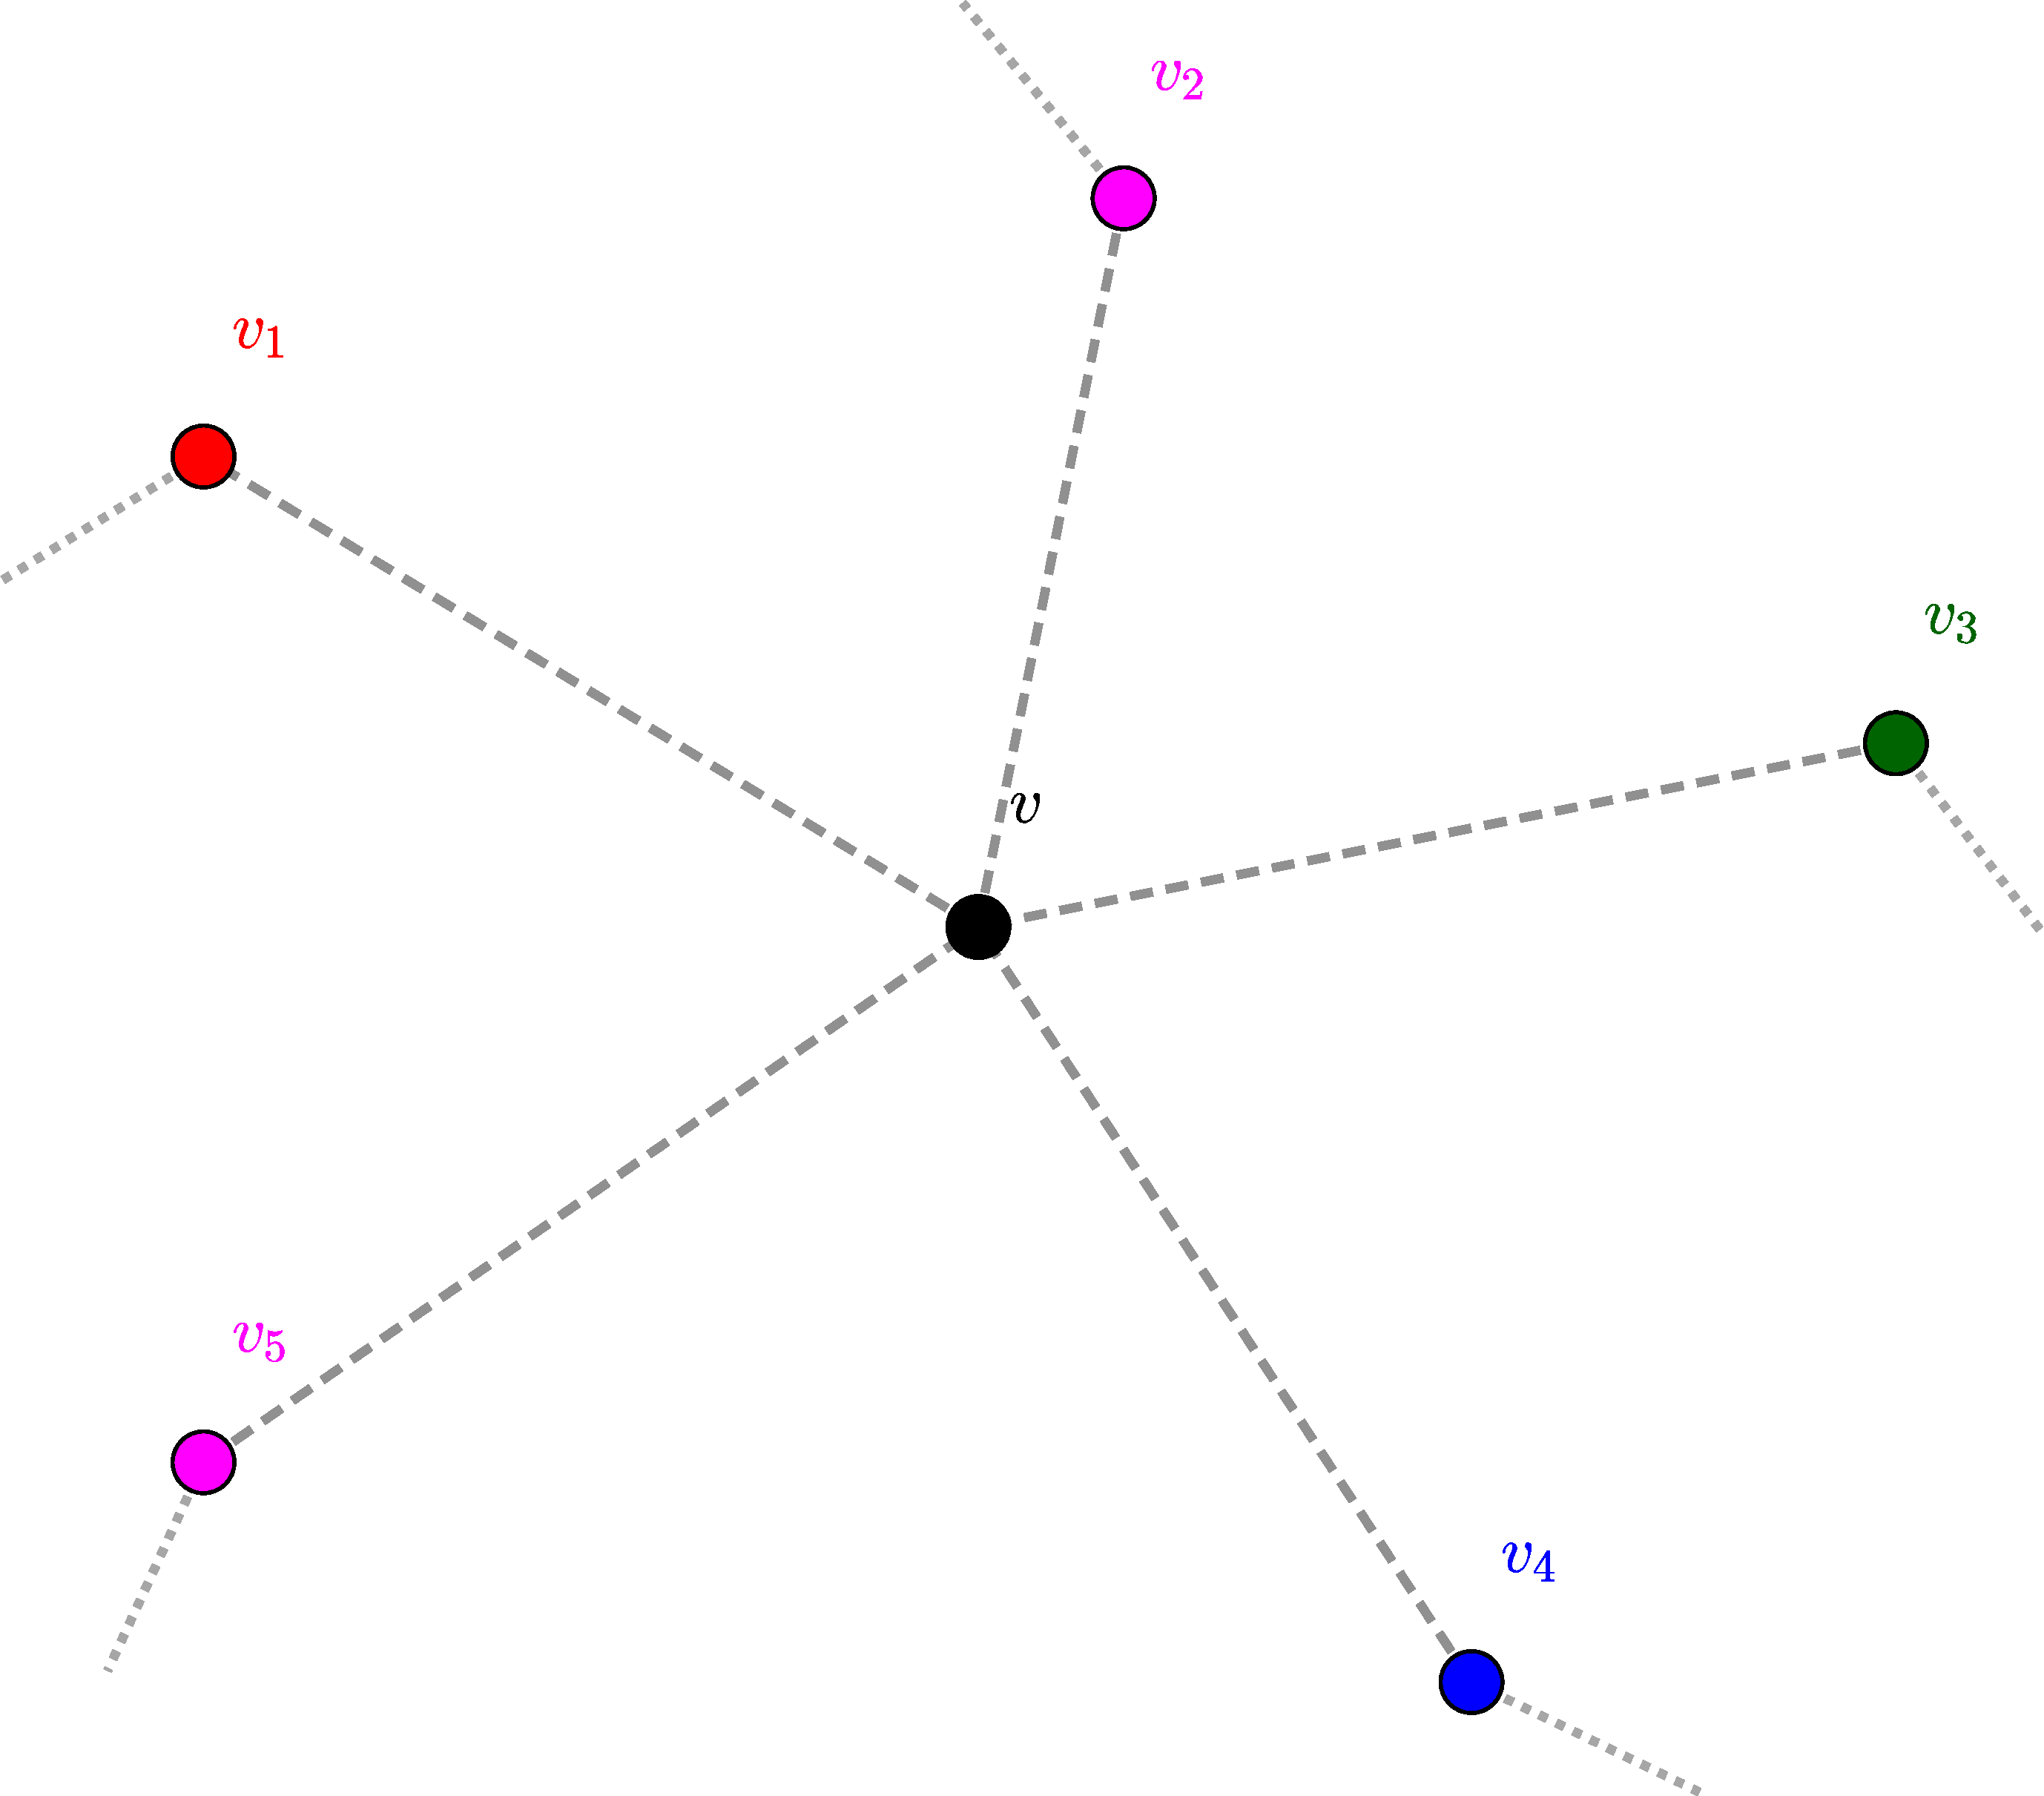
\includegraphics[width=\textwidth]{img/case1_first.pdf}
\caption{Diagram of $N(v) \subseteq H_{n}$}
\label{fig:case1_first}
\end{subfigure}
\begin{subfigure}[H]{0.49\textwidth}
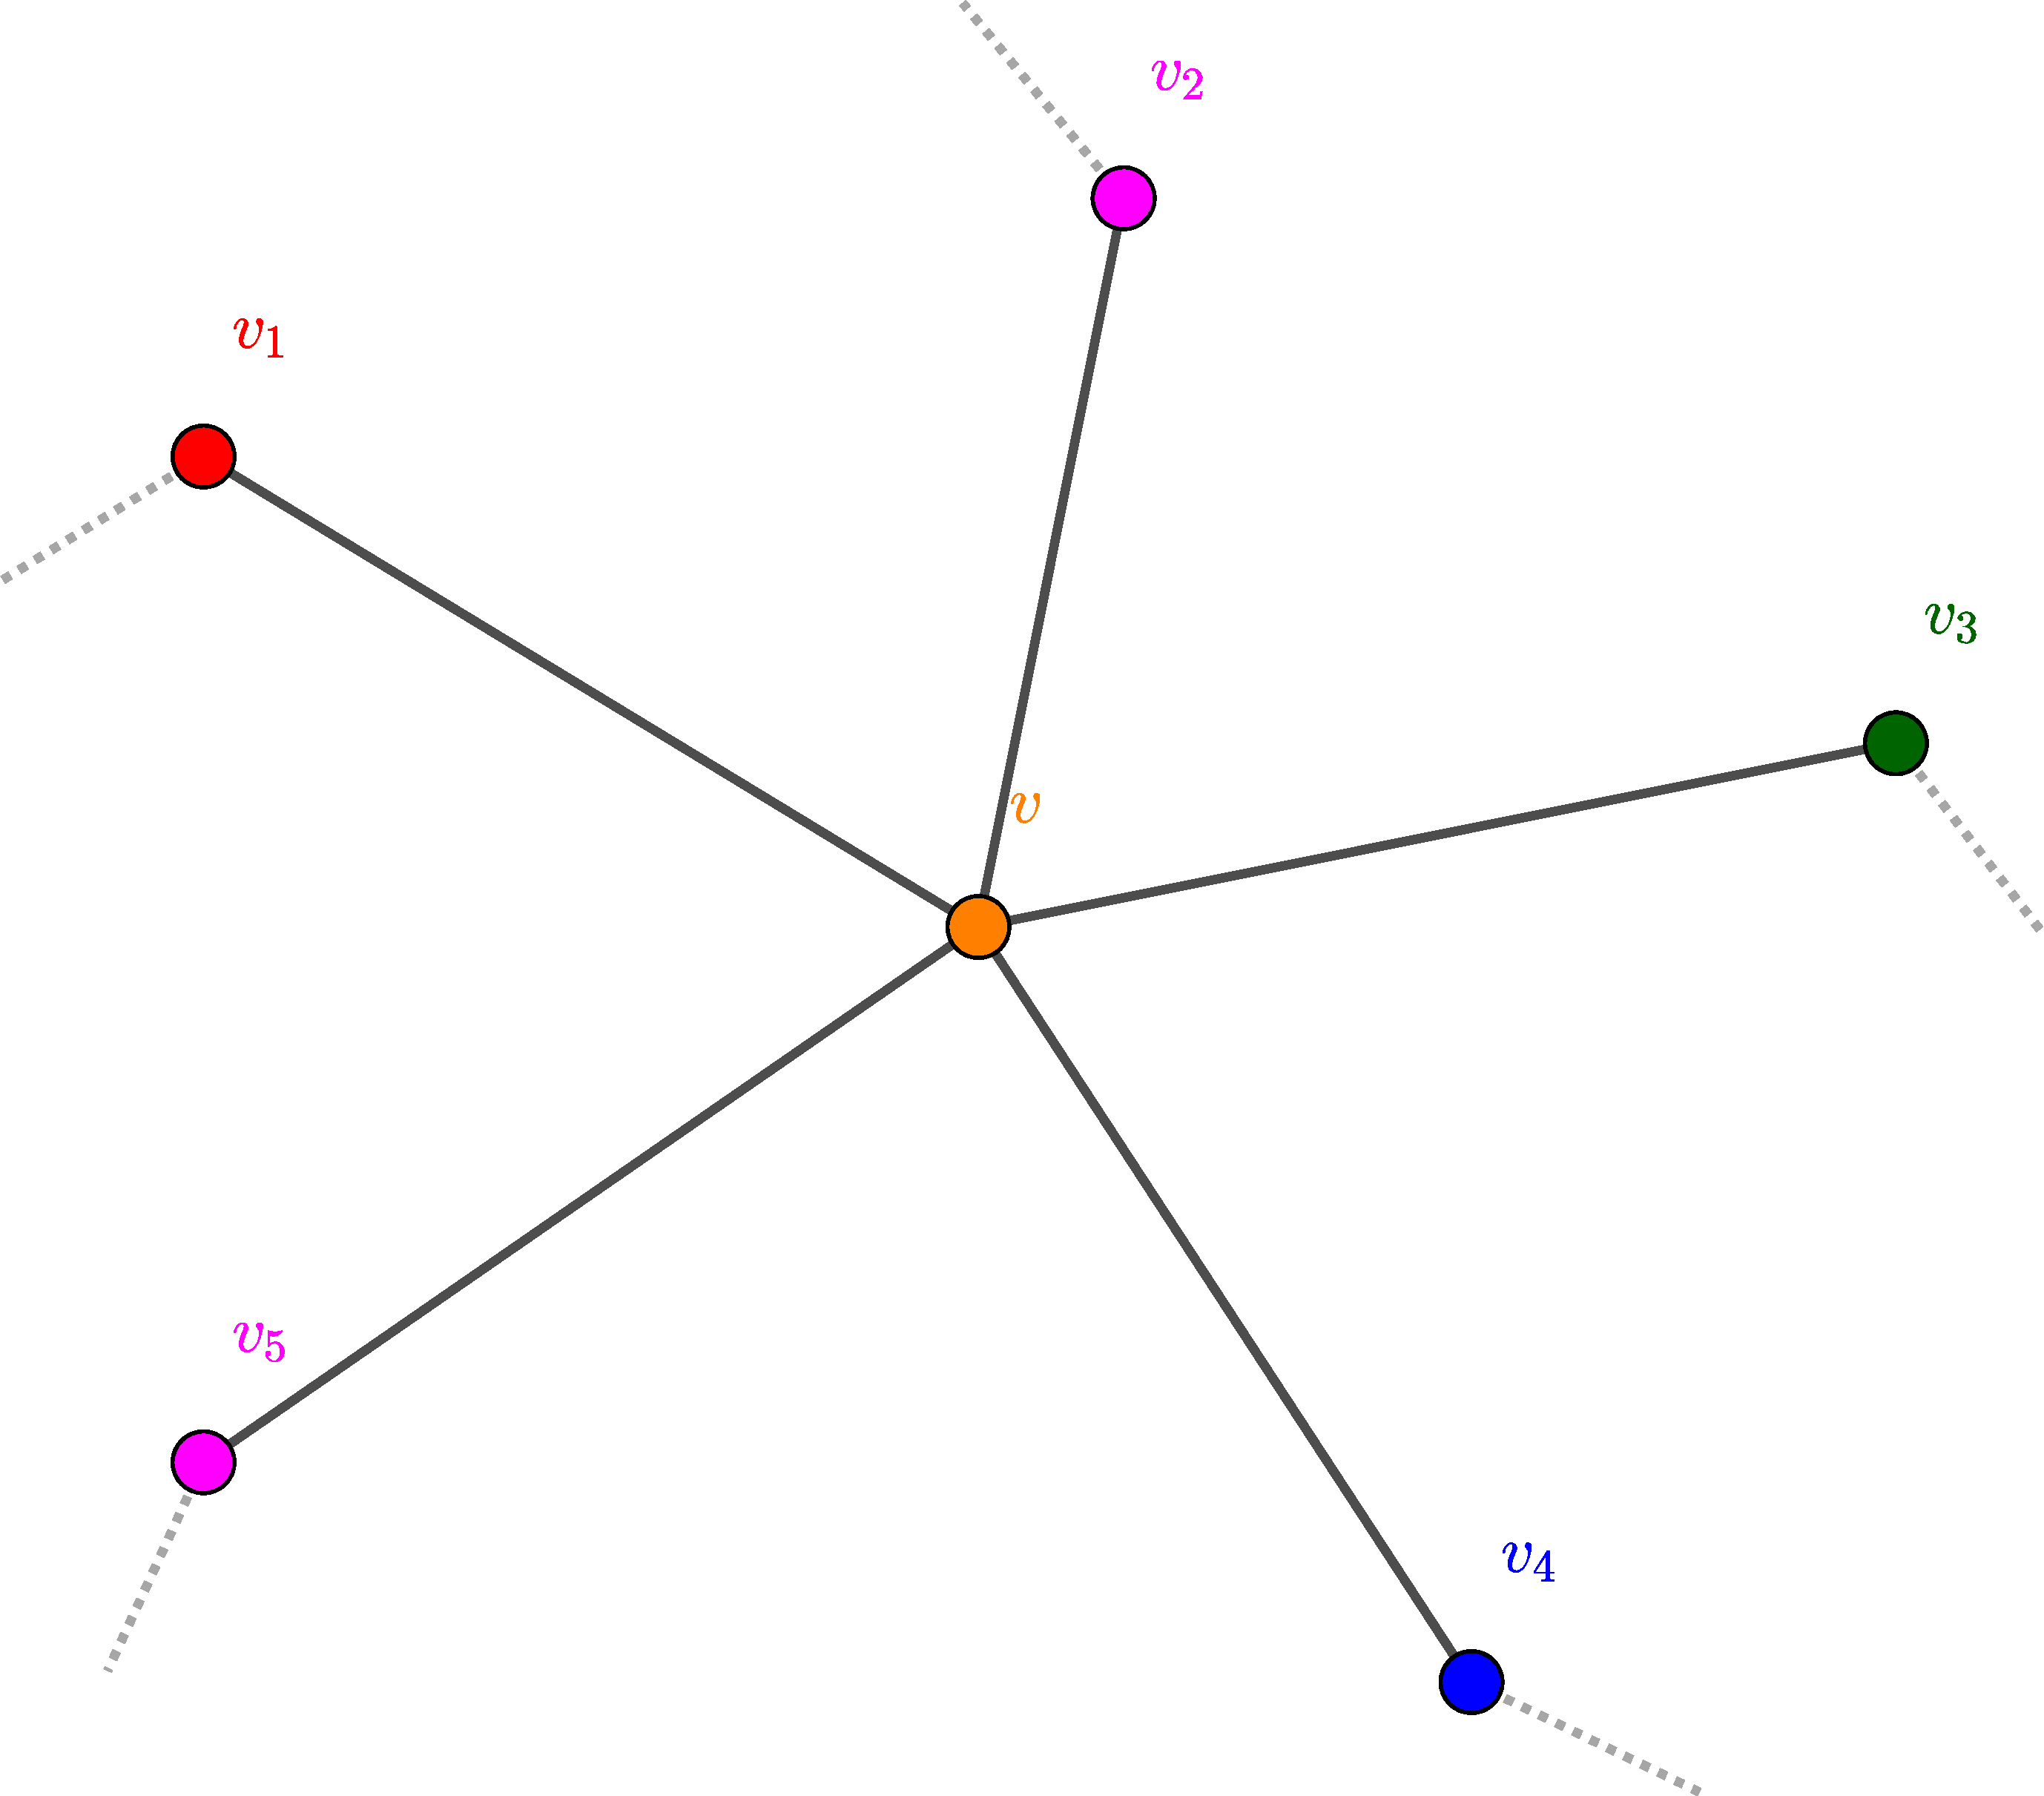
\includegraphics[width=\textwidth]{img/case1_second.pdf}
\caption{Diagram of $N(v) \subseteq G_{n + 1}$}
\label{fig:case1_second}
\end{subfigure}
\caption{Graph focussed around $N(v)$. The dotted lines represent arbitrary edges, whereas the vertices connected by the dashed edge are disjoint}
\end{figure}

$\phantom{x}$ \\
\textbf{case 2}: $|\{c(v_{i}) : v_{i} \in N(v)\}| = 5$

Since all vertices of $v$ are uniquely coloured, we cannot construct $G_{n + 1}$ such that it has a 5-colouring. We must reduce the colouring of $H_{n}$ so $v$ can be assigned the missing colour. For this let us consider a subgraph $H_{i, j} \subset H_{n}$, where $c(v_{i})$ and $c(v_{j})$ are the only possible colourings. This allows us to generalise the graph in such a way that vertices can be assigned different colours while maintaining a 5-colouring. Let us arbitrarily consider the vertices $v_{1}$ and $v_{3}$ from the previous illustration with $H_{1, 3} \subset H_{n}$. We now consider two more cases: \\
\textbf{case 2a}: Suppose $v_1$ and $v_3$ are not connected by a path in $H_{n}$

All vertices $v_i, v_j \in V(H_{i, j})$ where $c(v_i) \not = c(v_j)$ can be swapped with respect to each other without the need to modify the colouring of any other vertices outside of $H_{i, j}$. Since both $v_1, v_3 \in V(H_{1, 3})$, we are allowed to set $c(v_1) \defeq c(v_3)$ (or vice versa), such that $G_{n + 1} \defeq H_{n} \cup \{v\}$ and $v$ gets assigned the missing colour (as explained in case 1).

\begin{figure}[H]
\centering
\begin{subfigure}[H]{0.49\textwidth}
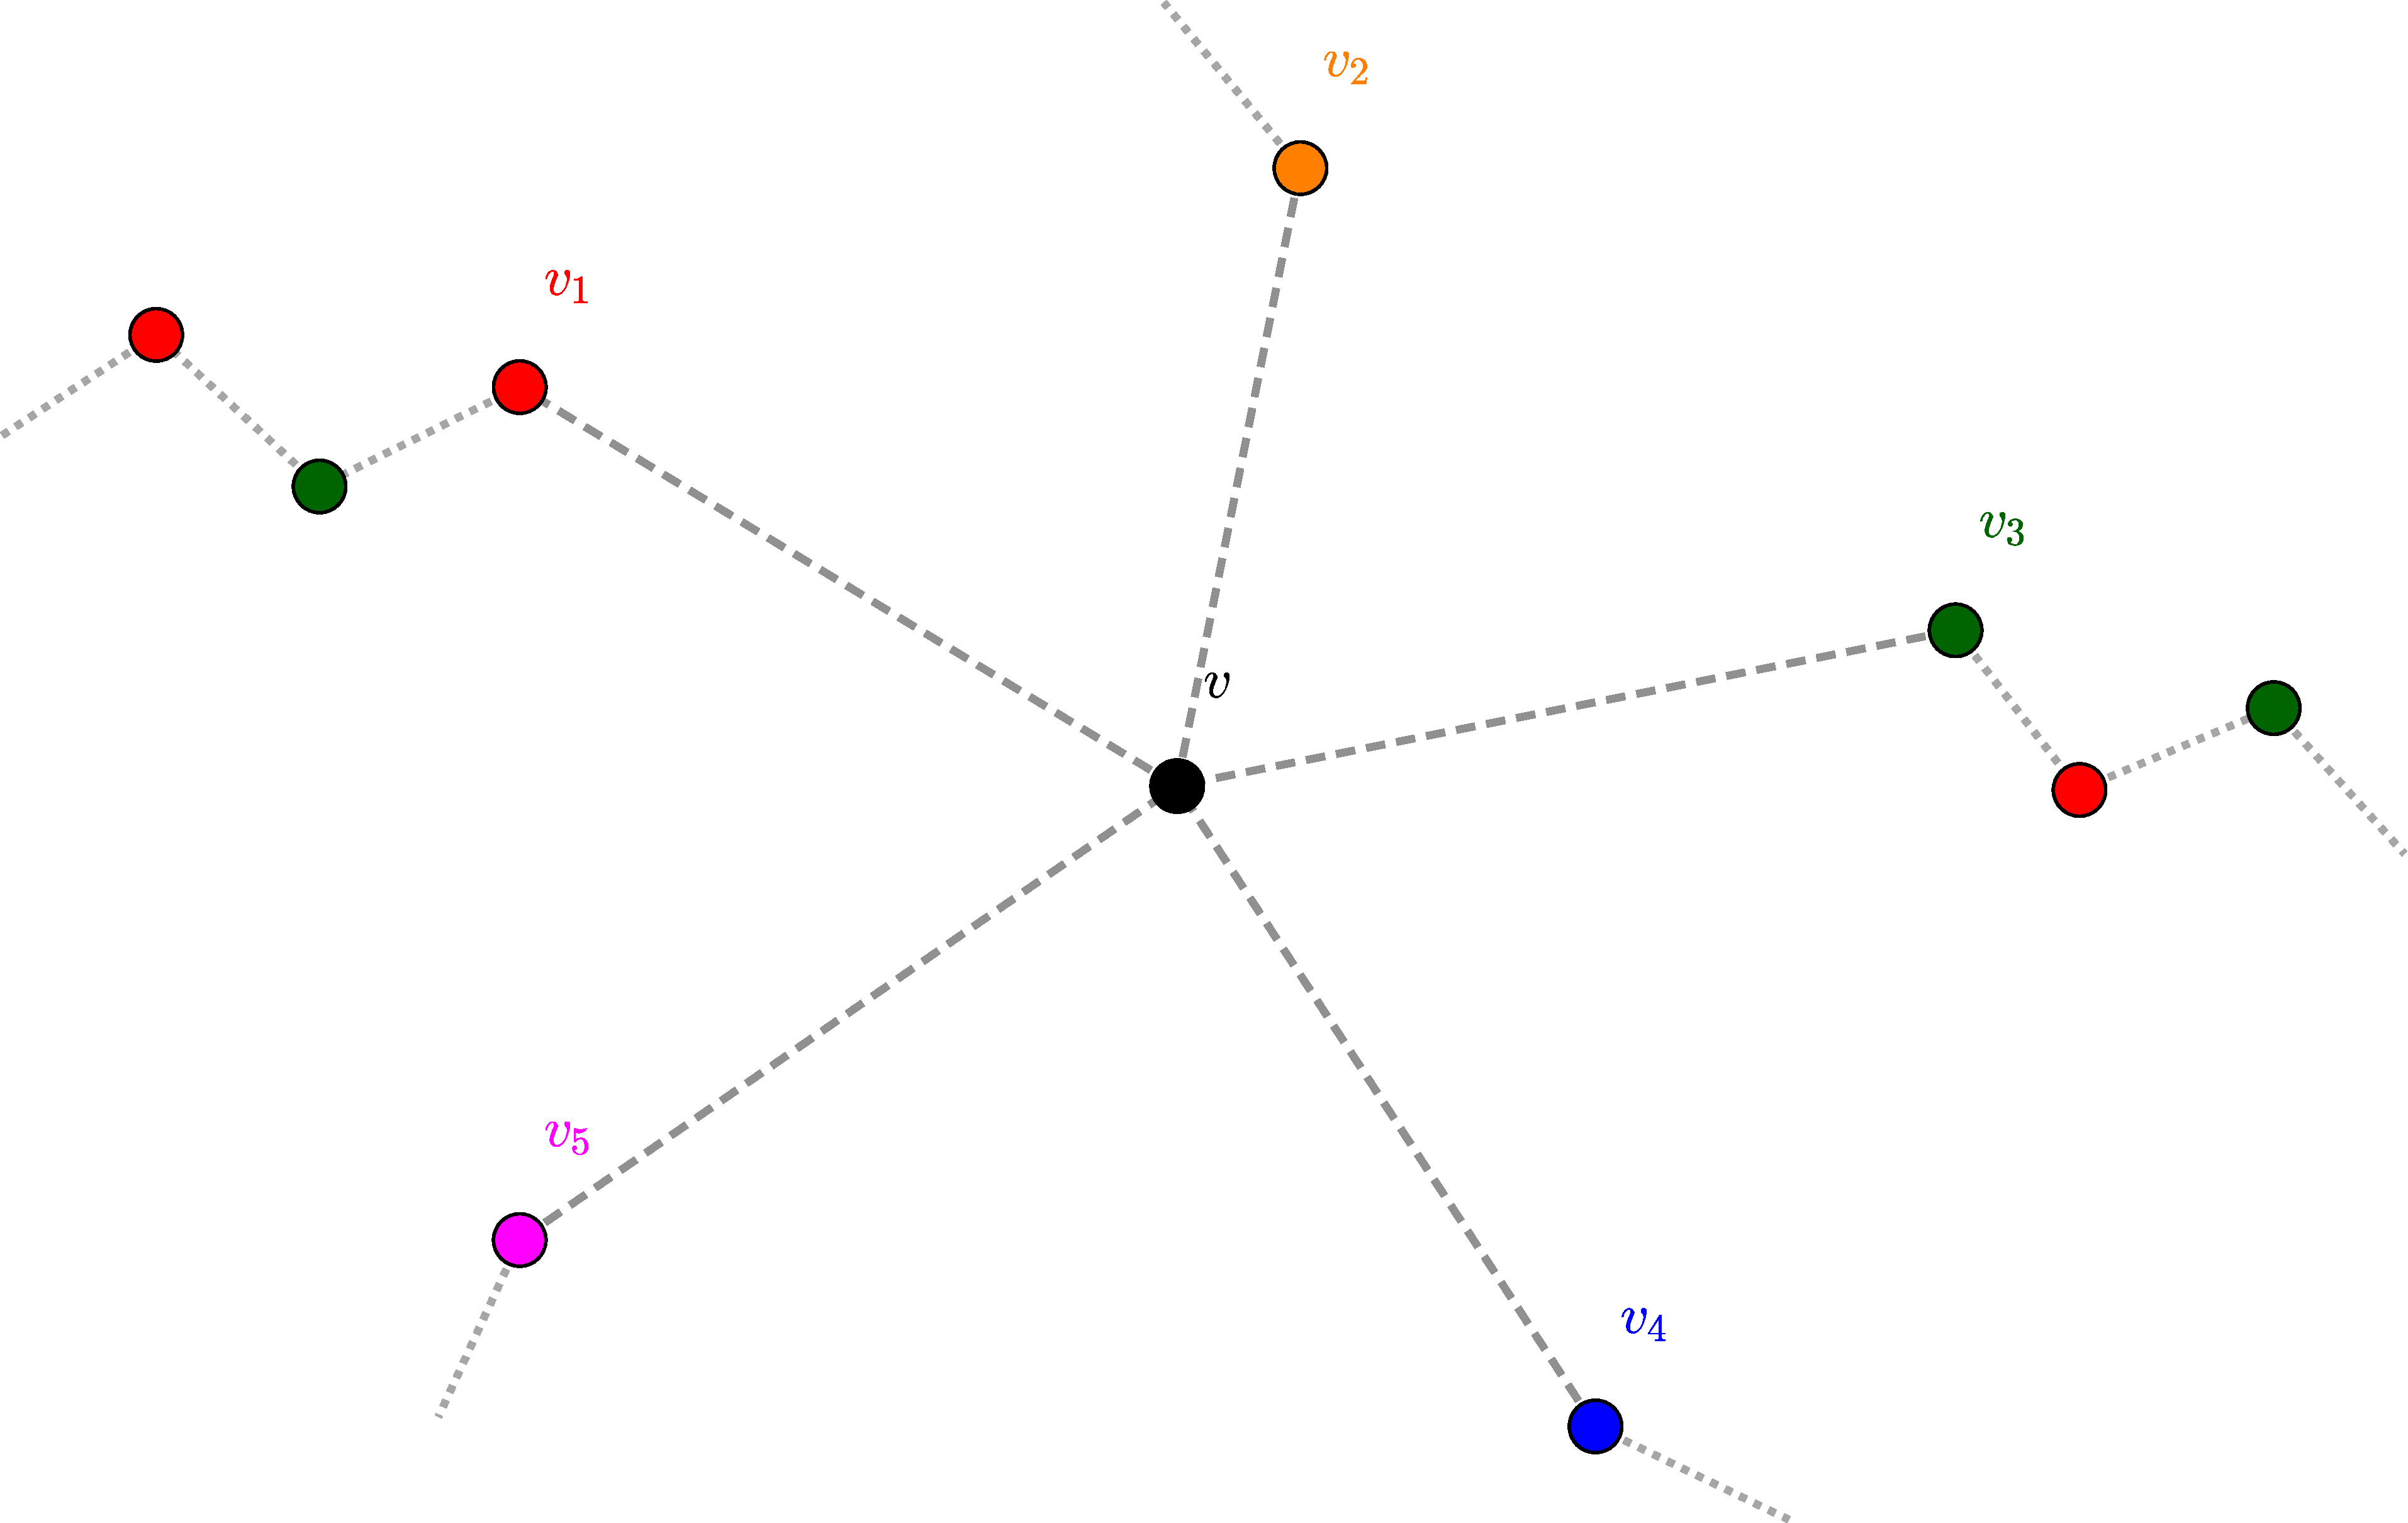
\includegraphics[width=\textwidth]{img/case2a_first.pdf}
\caption{Diagram of $N(v) \subseteq H_{n}$}
\label{fig:case2a_first}
\end{subfigure}
\begin{subfigure}[H]{0.49\textwidth}
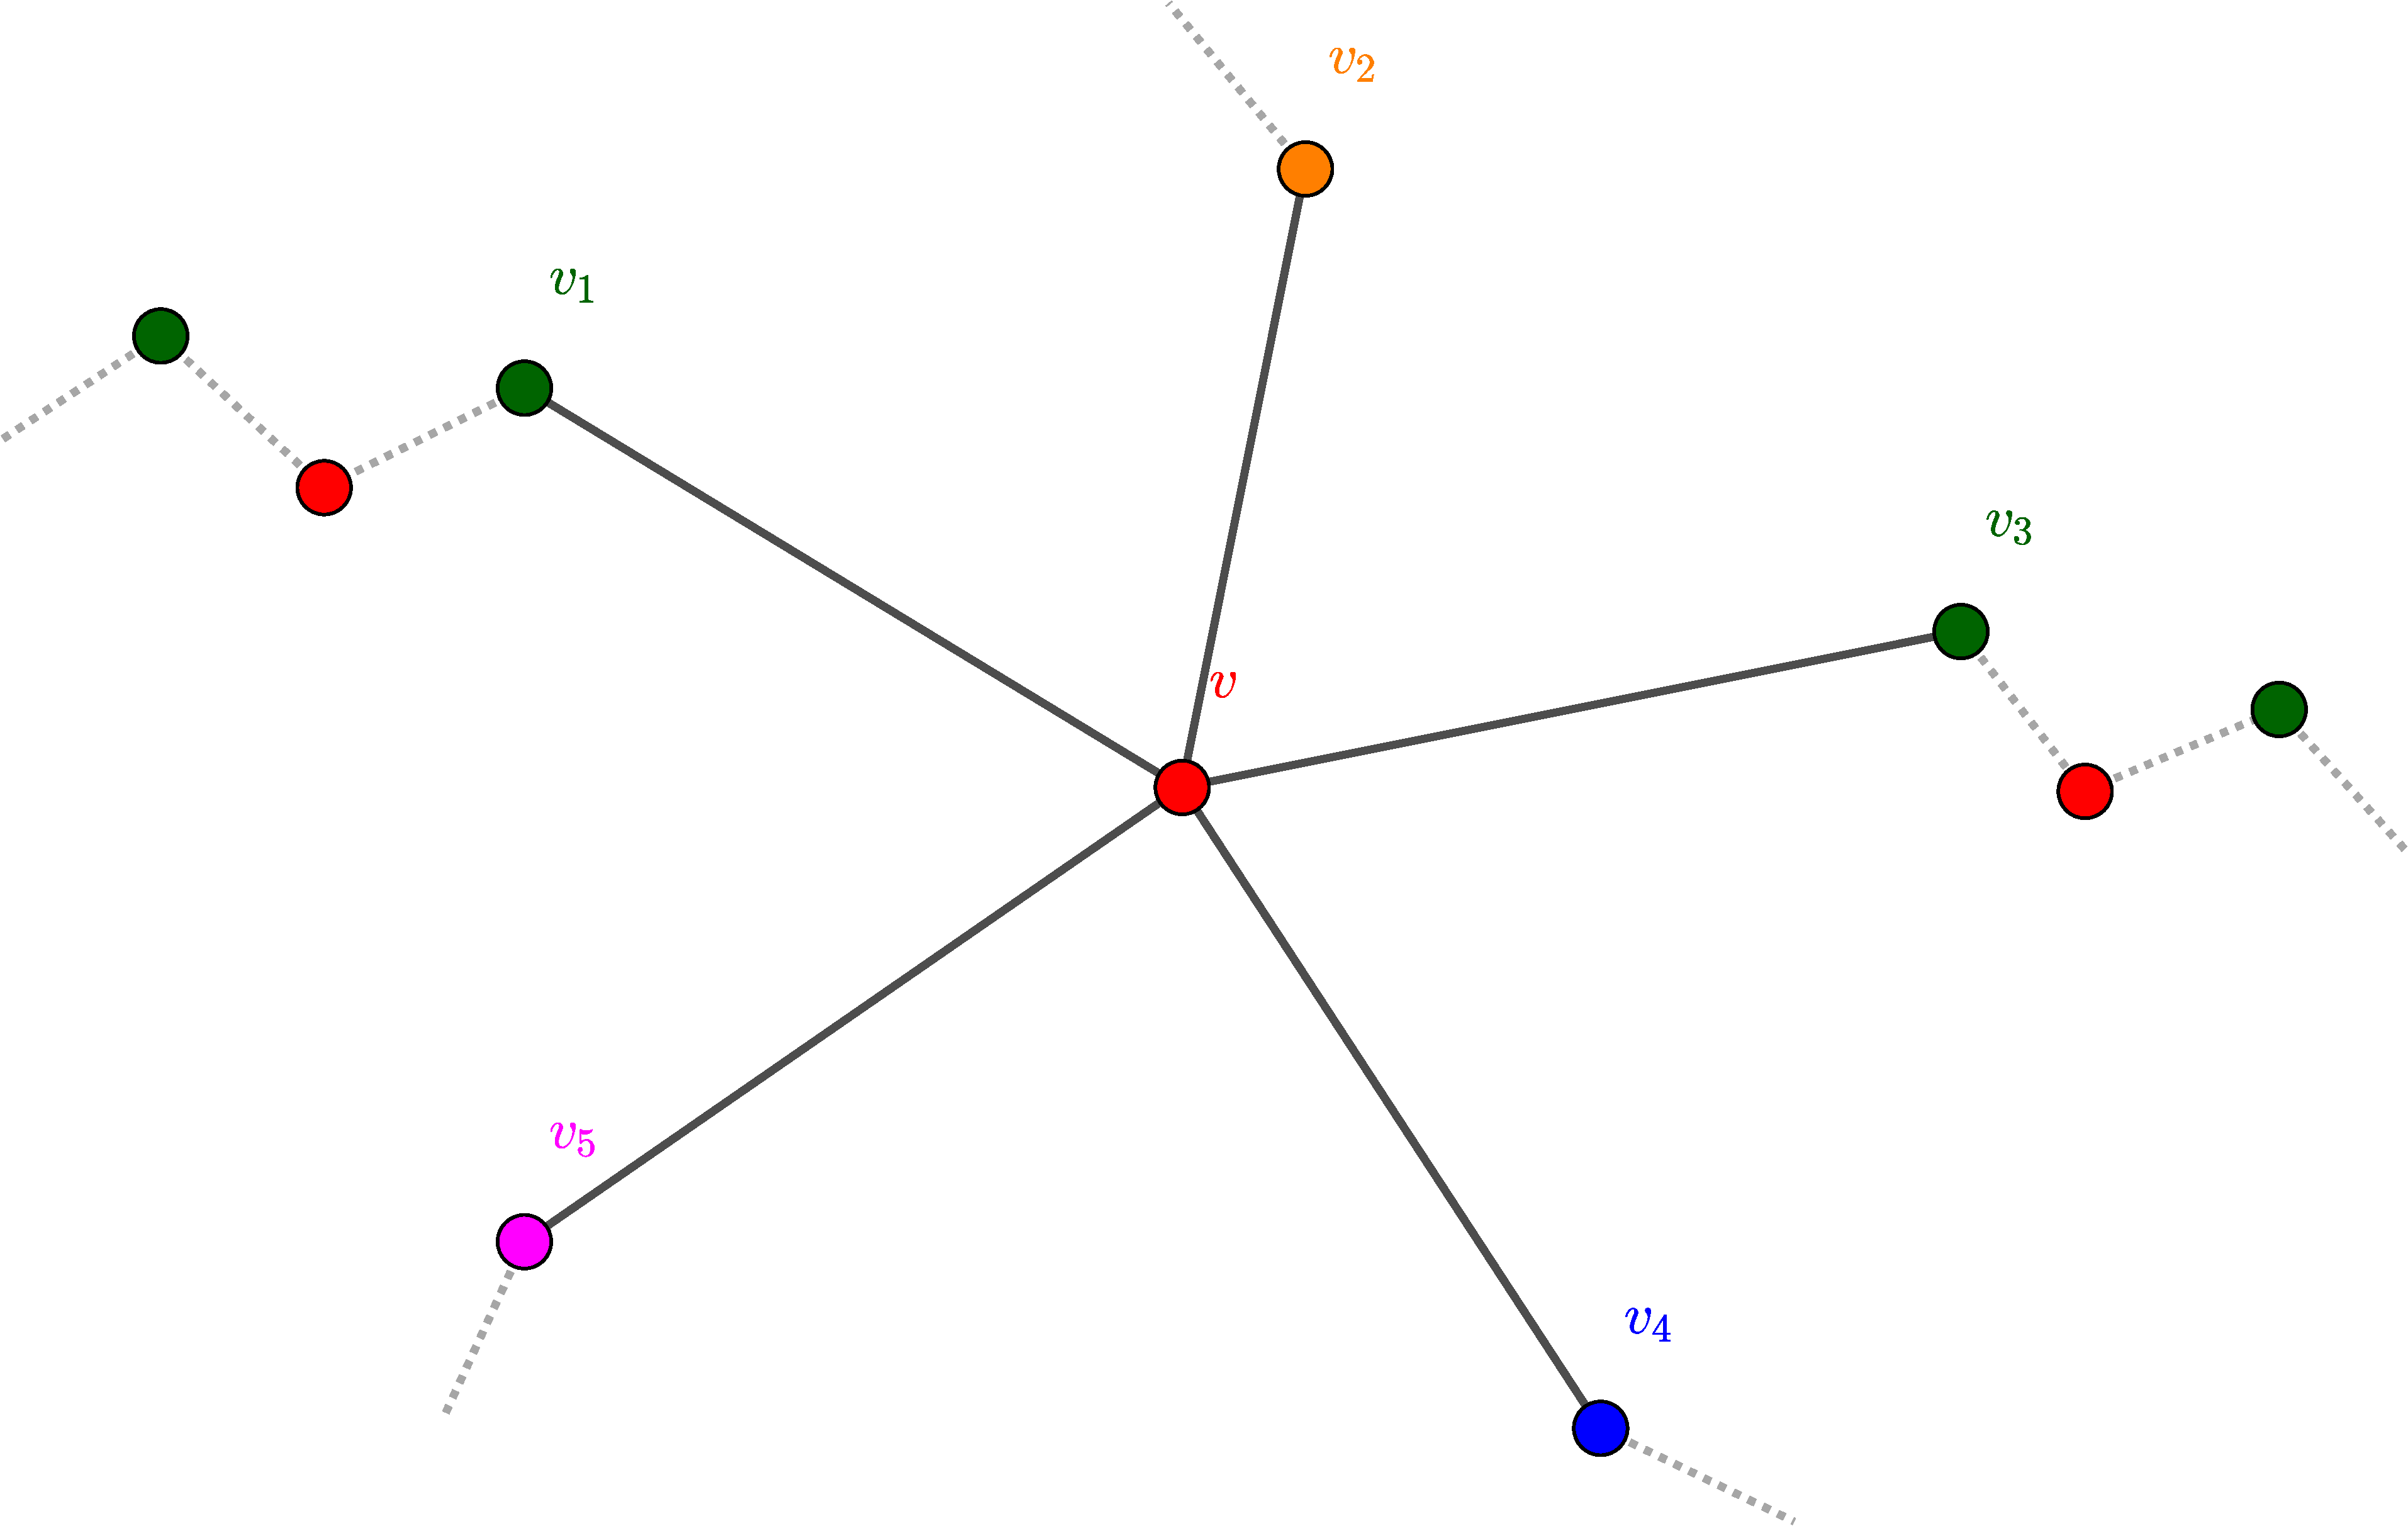
\includegraphics[width=\textwidth]{img/case2a_second.pdf}
\caption{Diagram of $N(v) \subseteq G_{n + 1}$}
\label{fig:case2a_second}
\end{subfigure}
\caption{Comparison of the planar graph before and after recolouring and union of $v$}
\end{figure}

$\phantom{x}$ \\
\textbf{case 2b}: Suppose $v_1$ and $v_3$ are connected by a path in $H_{n}$

Here the path of vertices connecting $v_{1}$ and $v_{3}$ in $H_{1,3} \cup \{v\}$ forms a cycle which contains $v_{2}$. We can safely assume that by our construction of $H_{1,3}$, the vertices $v_{2}$ and $v_{4}$ cannot be connected by a path in $H_{2,4}$, since this would disrupt the planarity of the graph $H_{n}$ (by intersecting edges). Because of this, $c(v_{2}) \defeq c(v_{4})$ (as in case 2a). Therefore $G_{n + 1} \defeq H_{n} \cup \{v\}$ and $v$ gets assigned the missing colour.

\begin{figure}[H]
\centering
\begin{subfigure}[H]{0.49\textwidth}
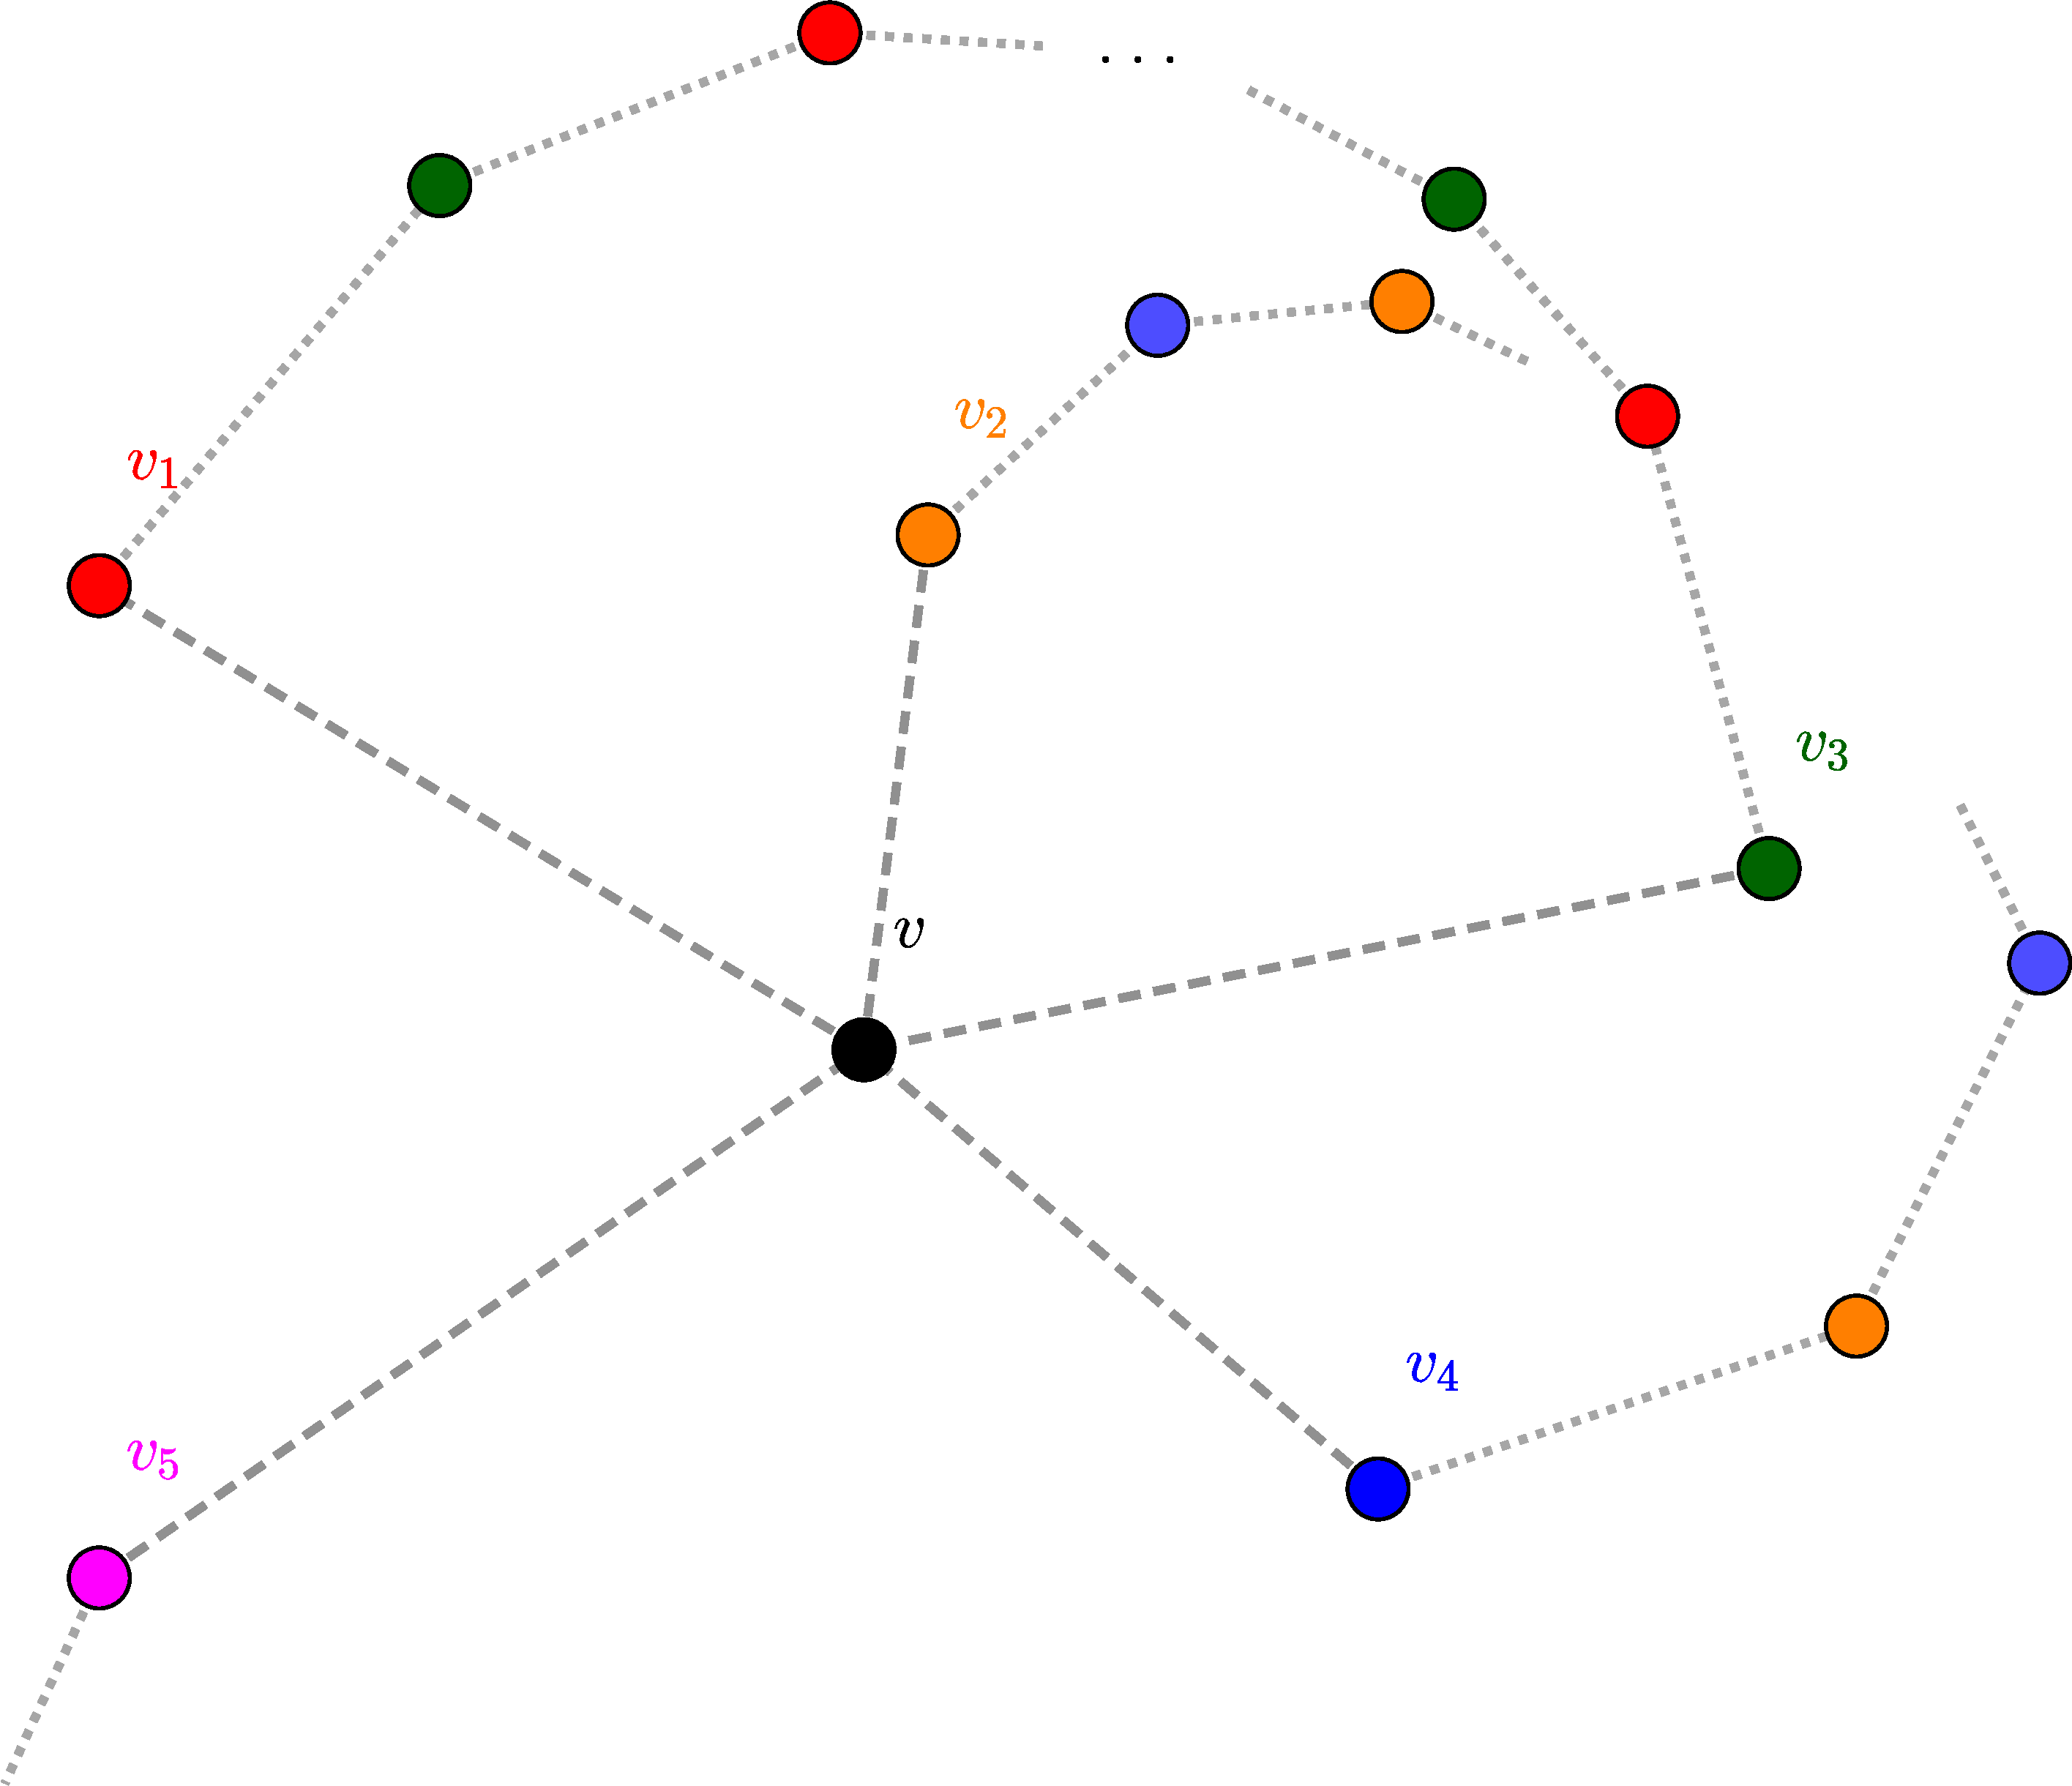
\includegraphics[width=\textwidth]{img/case2b_first.pdf}
\caption{Diagram of $N(v) \subseteq H_{n}$}
\label{fig:case2a_first}
\end{subfigure}
\begin{subfigure}[H]{0.49\textwidth}
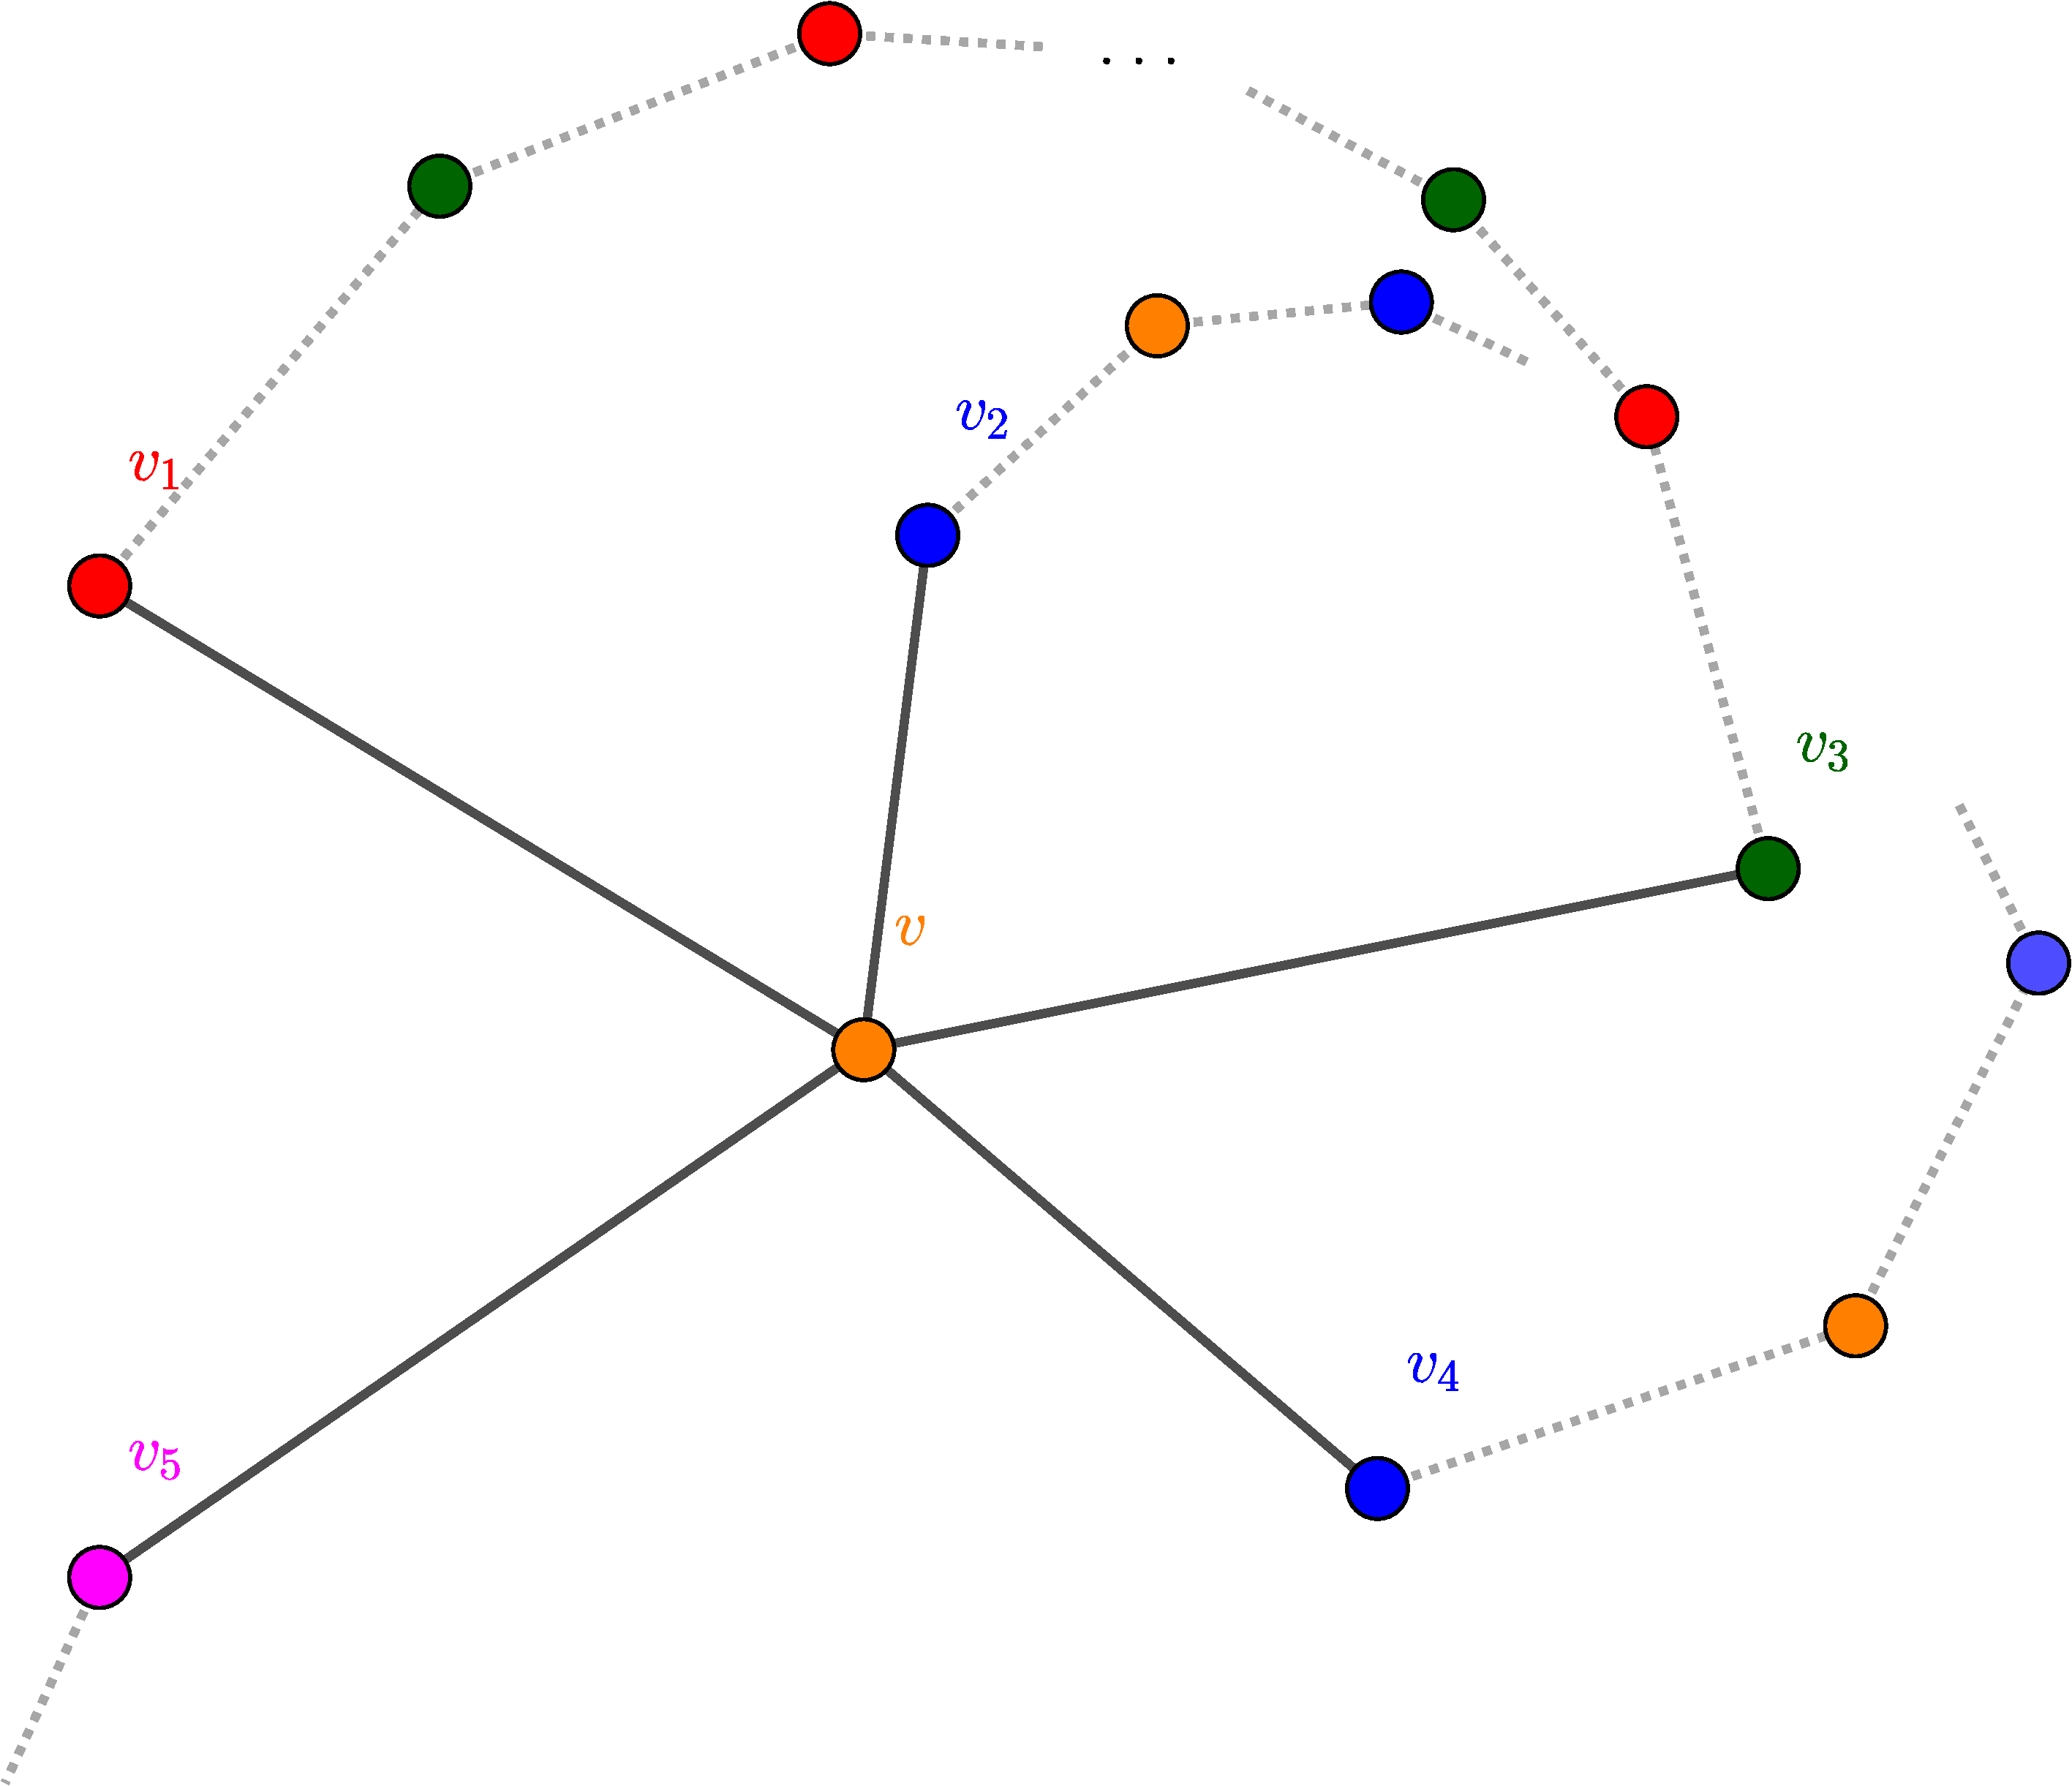
\includegraphics[width=\textwidth]{img/case2b_second.pdf}
\caption{Diagram of $N(v) \subseteq G_{n + 1}$}
\label{fig:case2a_second}
\end{subfigure}
\caption{Comparison of the planar graph before and after recolouring and the union of $v$}
\end{figure}

Since we can always find a way to recolour $H_{n}$ so that $H_{n} \cup \{v\} \eqdef G_{n + 1}$ is 5-colourable, by the principle of mathematical induction, $G_{n}$ is 5-colourable $\forall n \in \mathbb{N}$
\end{proof}

\nocite{*}
\pagebreak
\printbibliography

\end{document}
